\documentclass[12pt]{article}

\usepackage{graphicx}
\usepackage{listings}
\usepackage{color}
\definecolor{dkgreen}{rgb}{0,0.6,0}
\definecolor{gray}{rgb}{0.5,0.5,0.5}
\definecolor{mauve}{rgb}{0.58,0,0.82}
\lstdefinestyle{matlab}{
  language=Matlab,
  xleftmargin=\parindent,
  aboveskip=3mm,
  belowskip=3mm,
  showstringspaces=false,
  columns=flexible,
  basicstyle={\small\ttfamily},
  numbers=left,
  numberstyle=\tiny\color{gray},
  keywordstyle=\color{blue},
  commentstyle=\color{dkgreen},
  stringstyle=\color{mauve},
  breaklines=true,
  breakatwhitespace=true,
  tabsize=3
}
\lstdefinestyle{c}{
  language=C,
  xleftmargin=\parindent,
  aboveskip=3mm,
  belowskip=3mm,
  showstringspaces=false,
  columns=flexible,
  basicstyle={\small\ttfamily},
  numbers=left,
  numberstyle=\tiny\color{gray},
  keywordstyle=\color{blue},
  commentstyle=\color{dkgreen},
  stringstyle=\color{mauve},
  breaklines=true,
  breakatwhitespace=true,
  tabsize=3
}
\lstdefinestyle{bash}{
  language=bash,
  xleftmargin=\parindent,
  aboveskip=3mm,
  belowskip=3mm,
  showstringspaces=false,
  columns=flexible,
  basicstyle={\small\ttfamily},
  numbers=none,
  numberstyle=\tiny\color{gray},
  keywordstyle=\color{blue},
  commentstyle=\color{dkgreen},
  stringstyle=\color{mauve},
  breaklines=true,
  breakatwhitespace=true,
  tabsize=3
}
\usepackage{multicol}
\usepackage[a4paper, total={6in, 8.75in}]{geometry}
\usepackage{fancyhdr}
\usepackage{lastpage}
\usepackage{hyperref}
\usepackage{framed}
\usepackage{enumitem}
\usepackage{amsmath}
\usepackage{float}
\usepackage{empheq}
\usepackage{tabularx}
\usepackage{arydshln}
\usepackage{lipsum}
\usepackage{wrapfig}
\usepackage{titlesec}
\usepackage{ amssymb }
\usepackage{cases}
\usepackage[utf8]{inputenc}
\usepackage[english]{babel}
 
\usepackage[nottoc]{tocbibind}

\newcommand\scalemath[2]{\scalebox{#1}{\mbox{\ensuremath{\displaystyle #2}}}}
\newcommand\tab[1][1cm]{\hspace*{#1}}

\pagestyle{fancy}
\lhead{Matt Pascoe}
\rhead{Flyback Converter Design}
\cfoot{\thepage\ / \pageref{LastPage}}

\begin{document}

%Title
\title{RTL-SDR Radio}
\author{Matt Pascoe}
\maketitle
\newpage

\tableofcontents 
\listoffigures
\listoftables
\newpage 

\section{Theory}


\section{Design/Development}
This section of the report describes the method used to enable to RTL2832u SDR to receive the signal and process the received information to provide audio output.\\
This report is based primarily off of the work done in my university course at The University of Queesnland in COMS4105 and the ETSI EN 300 401 \cite{etsi} report.

\subsection{Setting up the RTL2832u}
This report will detail the method used for the following operating systems (OS).
\subsubsection{Windows 10}
\textbf{Installing Drivers}
\begin{enumerate}
	\item Get \href{http://zadig.akeo.ie/}{Zadig}
	\item Install Zadig
	\item Plug in USB tuner and open ``Zadig" to install USB drivers.\\ \textbf{NOTE:} Ensure that `List all devices' option is enabled under the Options tab.
	\begin{figure}[H]
		\centering
	    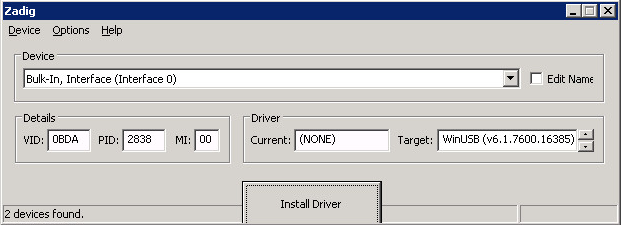
\includegraphics[width=0.8\textwidth]{install_win10-s1.png}
		\caption{Zadig without USB driver configured}
		\label{fig:install_win10-s1}
	\end{figure} 
	\item Select Device and WinUSB driver and click `Install Driver'
	\begin{figure}[H]
		\centering
	    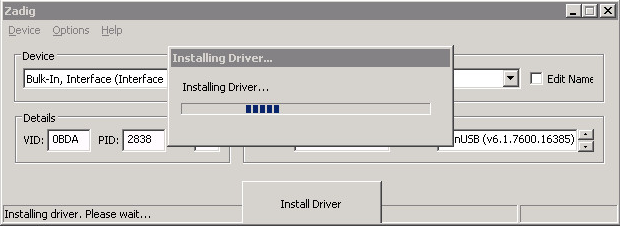
\includegraphics[width=0.8\textwidth]{install_win10-s2.png}
		\caption{After clicking `Install Driver'}
		\label{fig:install_win10-s2}
	\end{figure} 
	\begin{figure}[H]
		\centering
	    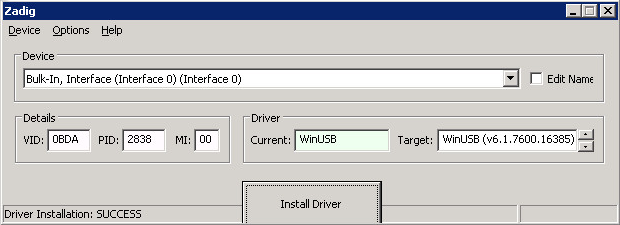
\includegraphics[width=0.8\textwidth]{install_win10-s3.png}
		\caption{After installing the correct driver (Note: WinUSB is selected)}
		\label{fig:install_win10-s3}
	\end{figure} 
	\item Get the `pre-built' command-line binaries from \href{http://sdr.osmocom.org/trac/attachment/wiki/rtl-sdr/RelWithDebInfo.zip}{here}
	\item Extract the files and navigate to them using the command line (Start > Run > CMD)
\end{enumerate}
\textbf{Testing RTL-SDR Device}\\
The RTL2832u can be tested using the following command through the command line:
\lstset{escapechar=@,style=bash}
\begin{lstlisting}
rtl_test -t
\end{lstlisting}
Which if it is working correctly it should return:\\[10cm]
\begin{lstlisting}
Found 1 device(s):		0:		ezcap USB 2.0 DVB-T/DAB/FM dongle
Using device 0: ezcap USB 2.0 DVB-T/DAB/FM dongle Found Rafael Micro R820T tuner
Supported gain values (29): 0.0 0.9 1.4 2.7 3.7 7.7 8.7 12.5 14.4 15.7 16.6 19.7 20.7 22.9  25.4 28.0 29.7 32.8 33.8 36.4 37.2 38.6 40.2 42.1 43.4 43.9 44.5 48.0 49.6
No E4000 tuner found, aborting.
\end{lstlisting}
\textbf{Capturing Data}
To capture data without any additional programs we cna use the following binary in the command line:
\begin{lstlisting}
rtl_sdr -s 2e6 -f 110.9e6 -n 2e6 dump.bin
\end{lstlisting}
Where the previous examples will capture 2 million samples (-n = number), at a sample rate of 2 megasamples/second (-s) and with a center frequency of 110.9 MHz (-f). Samples will be captured into dump.bin\\[3mm]
\textbf{Displaying the Data}
The tool for displaying data that is used in the report is \href{http://airspy.com/download/}{SDRSharp} which allows for displaying the data in two different ways; spectral density and a waterfall map.\\
To get SDR sharp working first run the following in the command line:
\begin{lstlisting}
rtl_tcp
\end{lstlisting}
then open SDRSharp and connect to the TCP server. Have fun!



%-------------------------------------------------
% Actual document
%-------------------------------------------------
\newpage
\section{Processing RTL-SDR}
\subsection{Processing RTL2832u with C}


\newpage
\section{AM Receiver}



\newpage
\section{FM Receiver}
\subsection{Background - FM Spectrum}

\subsection{FM Demodulation}


\subsection{Processing FM}

\begin{figure}[H]
	\centering
	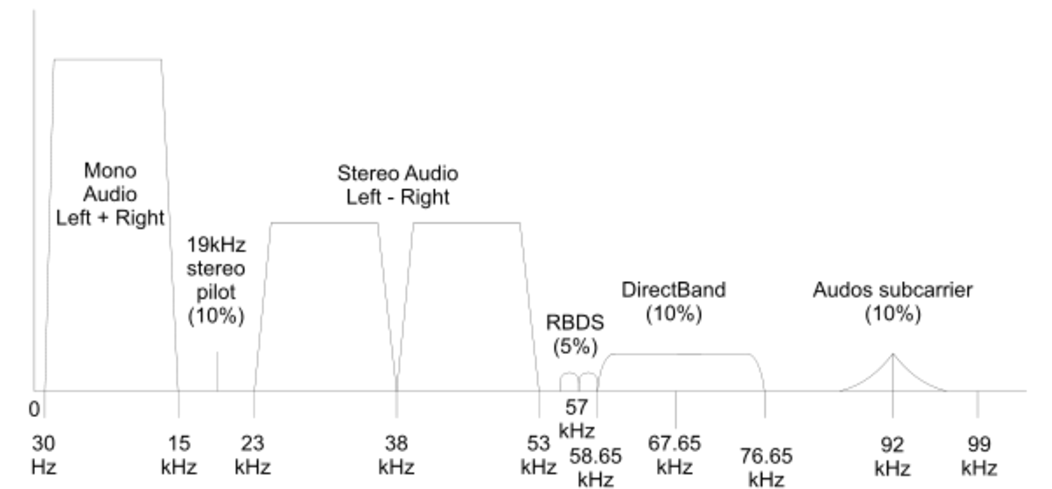
\includegraphics[width=0.8\textwidth]{FM_demodulated.png}
	\caption{FM Demodulated Signal}
	\label{fig:fm:demod-sig}
\end{figure}
For this document it will look at the Mono Audio (L+R), $19$KHz stereo pilot, Stereo Audio (L-R) and the Radio Broadcast Data System (RBDS).

\subsubsection{Audio - Mono}

\subsubsection{Audio - Stereo} 

\subsubsection{RBDS}











%-------------------------------------------------
% Bibliography
%-------------------------------------------------
\newpage
\begin{thebibliography}{9} 
\bibitem{etsi} 
ETSI EN 300 401 V1.4.1, European Broadcasting Union, 2006-01, 
\\\texttt{http://www.etsi.org/deliver/etsi\_en/300400\_300499/300401/01.04.01\_40/en\_300401v010401o.pdf}



\end{thebibliography}
\end{document}